\documentclass{article}[12pt,a4paper]
\usepackage[utf8]{inputenc}
\usepackage{caption}
\usepackage{amsmath} 
\usepackage{hyperref}
\usepackage{csquotes}
\usepackage{graphicx}

\hypersetup{
    colorlinks=true,
    linkcolor=blue,
    filecolor=magenta,      
    urlcolor=cyan,
}

\graphicspath{ {./} }

\title{A jófej és az írás}
\author{Rátki Barnabás}
\date{2020.08.02}

\begin{document}
\maketitle

A probléma a következő volt:
\begin{displayquote}
Parker és Brett pénzfeldobóst játszanak. Hány érme használata esetén lesz a fejek száma 25\% valószínűséggel 3 darab? (Segítség:  lehet kísérletezéssel is kísérletezni, ez esetben mellékelje a mérési jegyzőkönyvet!)
\end{displayquote}

\section{Megoldás}

Legyen a használt pénzérmék száma $n$.

Így az összes lehetséges dobások száma: $2^n$. (Egy pénzérmét ha feldobunk 2 fajta eredménye lehet)\par
Azoknak a dobásoknak a száma ahol pontosan 3 fej van: ${n}\choose{3}$. (Hány fajta képpen tudunk ebből az n darabból kiválasztani a 3 fejet amit várunk.)\par

Tehát annak a valószínűsége, hogy pontosan 3 fej lesz megkapható úgy, hogy (Kedvező esetek száma ösztva az összes eset számával módszerrel) $$\frac{\frac{n!}{3!\cdot(n-3)!}}{2^n}$$ \par
A feladatnak csak egész megoldásai vannak ezért elég könnyen ábrázolni tudjuk ezt $n$ függvényében: 
\begin{center}
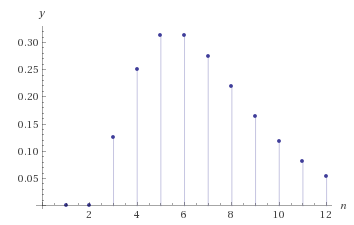
\includegraphics{graf1} 
\end{center}

A grafikonról leolvashatjuk, hogy a megoldás a \textbf{4} lesz mivel $n=4$ esetén a fenti kifejezés értéke $0.25$ (Tehát a valószínűség 25\%).

\end{document}
